\documentclass[xcolor=dvipsnames,notes]{beamer}
\usecolortheme[named=Brown]{structure}
\usetheme{default}
\setbeamertemplate{navigation symbols}{} 
\usepackage{tikz}
\usetikzlibrary{arrows,decorations.pathmorphing,backgrounds,positioning,fit}
\usetikzlibrary{datavisualization.formats.functions}
\usetikzlibrary{shapes}
\include{macro}
\usepackage{epsfig}
\usepackage{natbib}
\usepackage{graphicx}
\usepackage{multimedia}
\usepackage{verbatim}
\include{acmmacro}
\begin{document}
%\setbeamercolor{titlelike}{fg=gray,bg=white}
%\setbeamercolor{itemize item}{fg=gray,bg=white}
%\setbeamercolor{enumerate item}{fg=gray,bg=white}
%\setbeamercolor{block title}{fg=black,bg=white}
%==============================================
\title{TPG4190 Seismic data acquisition and processing \\
               Lecture 9: Processing}
\author{B. Arntsen}
\institute[NTNU]{
  NTNU\\
  Department of Geoscience and petroleum \\
  \texttt{borge.arntsen@ntnu.no}
}
\date{Trondheim fall 2021}
\begin{frame}
 \titlepage
\end{frame}
%
%==============================================
\begin{frame}{Overview}
%==============================================
\begin{itemize}
  \item Filters
   \item Basic processing sequence
   \item Basic+ processing sequence
   \item Basic++ processing sequence
  \end{itemize}
\end{frame}
%==============================================
\begin{frame}{Basic processing sequence}
%==============================================
\begin{enumerate}
  \item Input data
  \item Velocity analysis
  \item NMO + Stack
  \item Output result
\end{enumerate}
\end{frame}
%-------------------------------------------------
\begin{frame}{Seismic marine data acquisition}
%-------------------------------------------------
%
\begin{figure}
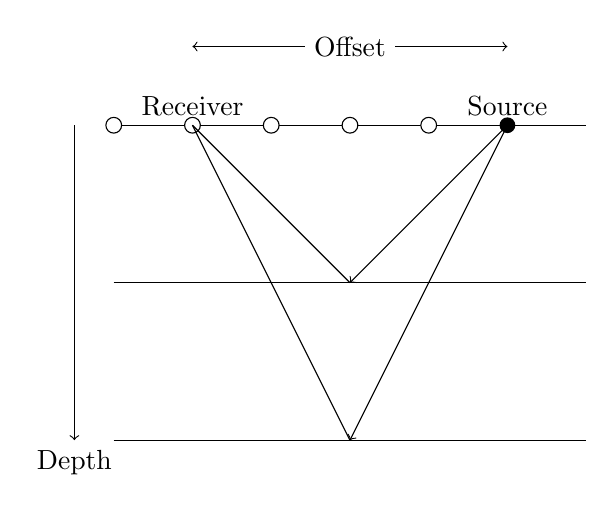
\begin{tikzpicture}
  \draw[->] (-0.5,4.0) -- (-0.5,0.0) node[below]{Depth} ;
  \draw[<->] (1.0,5.0) -- node[fill=white]{Offset} (5.0,5.0); 
  \draw (0.0,0.0) -- (6.0,0.0) ;
  \draw (0.0,2.0) -- (6.0,2.0) ;
  \draw (0.0,4.0) -- (6.0,4.0) ;
  \fill (5.0,4.0) node[above]{Source} circle (0.1) ;
  \fill[white] (0.0,4.0) circle (0.1) ;
  \draw (0.0,4.0) circle (0.1) ;
  \fill[white](1.0,4.0) circle (0.1) ;
  \draw (1.0,4.0) node[above]{Receiver}circle (0.1) ;
  \fill[white] (2.0,4.0) circle (0.1) ;
  \draw (2.0,4.0) circle (0.1) ;
  \fill[white] (3.0,4.0) circle (0.1) ;
  \draw (3.0,4.0) circle (0.1) ;
  \fill[white] (4.0,4.0) circle (0.1) ;
  \draw (4.0,4.0) circle (0.1) ;
  \draw[->] (5.0,4.0) -- (3.0,0.0) ;
  \draw (3.0,0.0) -- (1.0,4.0) ;
  \draw[->] (5.0,4.0) -- (3.0,2.0) ;
  \draw (3.0,2.0) -- (1.0,4.0) ;
\end{tikzpicture}
\label{fig:geom}
\end{figure}
\end{frame}
%
%-----------------------------------------
\begin{frame}{Schematic shot record}
%-----------------------------------------
%
\begin{figure}
\includegraphics[width=0.5\textwidth]{Fig/schemshot.pdf}
\end{figure}
%
\end{frame}
%----------------------------------------------
\begin{frame}{Real shot record}
%----------------------------------------------
%
\begin{figure}
\includegraphics[width=0.5\textwidth]{Fig/shotgath.pdf}
\end{figure}
%
\end{frame}
%-----------------------------------------
\begin{frame}{The cmp method}
%-----------------------------------------
%
\begin{figure}
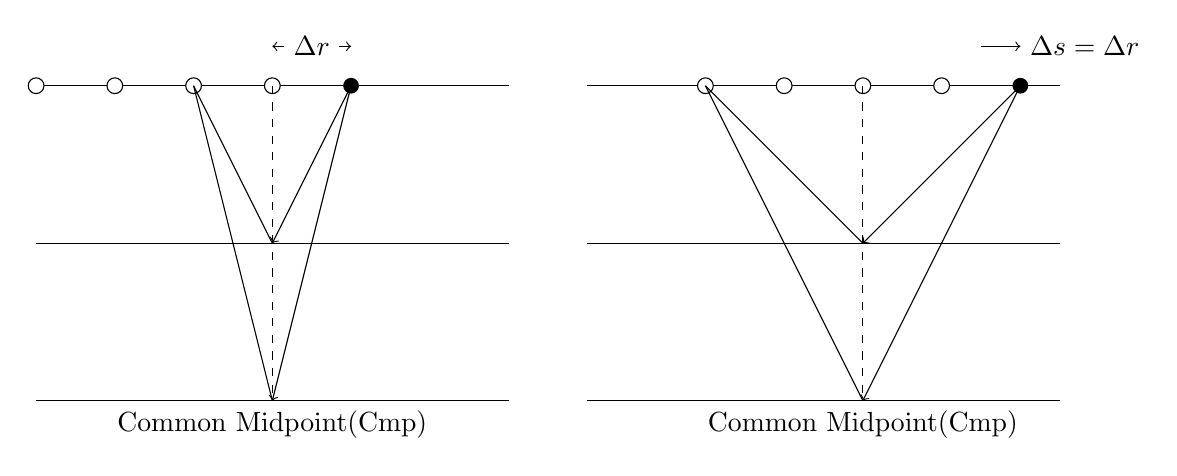
\begin{tikzpicture}
  \draw[<->] (3.0,4.5) -- node[fill=white]{$\Delta r$}(4.0,4.5); % Draw Delta r 
  \draw (0.0,0.0) -- (6.0,0.0) ;     %Draw Bottom reflector left display
  \draw (0.0,2.0) -- (6.0,2.0) ;     %Draw Middle reflector left display
  \draw (0.0,4.0) -- (6.0,4.0) ;     %Draw Surface left display
  \fill (4.0,4.0) circle (0.1) ;     %Draw source left display

  %Draw receivers on left display 

  \fill[white] (0.0,4.0) circle (0.1) ; 
  \draw (0.0,4.0) circle (0.1) ;
  \fill[white] (1.0,4.0) circle (0.1) ;
  \draw (1.0,4.0) circle (0.1) ;
  \fill[white] (2.0,4.0) circle (0.1) ;
  \draw (2.0,4.0) circle (0.1) ;
  \fill[white] (3.0,4.0) circle (0.1) ;
  \draw (3.0,4.0) circle (0.1) ;
 
  % Draw dashed vertical line and cmp text below bottom reflector left display
  \draw[dashed] (3.0,4.0) -- (3.0,0.0) node[below]{Common Midpoint(Cmp)} ;

  %Draw raypaths to bottom layer left display
  \draw[->] (4.0,4.0) -- (3.0,0.0) ; 
  \draw (3.0,0.0) -- (2.0,4.0) ;     

  %Draw raypaths to middle layer left display
  \draw[->] (4.0,4.0) -- (3.0,2.0) ;
  \draw (3.0,2.0) -- (2.0,4.0) ;

  \draw (7.0,0.0) -- (13.0,0.0) ; Draw bottom reflector right display
  \draw (7.0,2.0) -- (13.0,2.0) ; Draw middle reflector right display
  \draw (7.0,4.0) -- (13.0,4.0) ; Draw surface right display

  % Draw Delta s headline
  \fill (12.5,4.0) circle (0.1) ;
  \draw[->] (12.0,4.5) -- (12.5,4.5) node[right]{$\Delta s=\Delta r$};

  %Draw receivers on right display 
  \fill[white] (8.5,4.0)  circle (0.1) ;
  \draw (8.5,4.0)  circle (0.1) ;
  \fill[white] (9.5,4.0)  circle (0.1) ;
  \draw (9.5,4.0)  circle (0.1) ;
  \fill[white] (10.5,4.0) circle (0.1) ;
  \draw (10.5,4.0) circle (0.1) ;
  \fill[white] (11.5,4.0) circle (0.1) ;
  \draw (11.5,4.0) circle (0.1) ;

  %Draw raypaths to bottom layer
  \draw[->] (12.5,4.0) -- (10.5,0.0) ;
  \draw (10.5,0.0) -- (8.5,4.0) ;

  %Draw raypaths to middle layer
  \draw[->] (12.5,4.0) -- (10.5,2.0) ;
  \draw (10.5,2.0) -- (8.5,4.0) ;

  % Draw dashed vertical line and cmp text below bottom reflector left display
  \draw[dashed] (10.5,4.0) -- (10.5,0.0)node[below]{Common Midpoint(Cmp)} ;

\end{tikzpicture}
\label{fig:shotsgeom}
\end{figure}
%
\end{frame}
%--------------------------------------------
\begin{frame}{Common midpoint (cmp) gather}
%--------------------------------------------
\begin{figure}
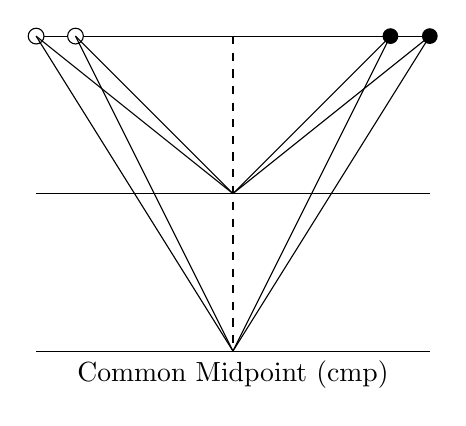
\begin{tikzpicture}
  \draw (0.0,0.0) -- (5.0,0.0) ;
  \draw (0.0,2.0) -- (5.0,2.0) ;
  \draw (0.0,4.0) -- (5.0,4.0) ;
  \fill[white] (0.0,4.0) circle (0.1) ;
  \draw (0.0,4.0) circle (0.1) ;
  \fill (5.0,4.0) circle (0.1) ;
  \fill[white] (0.5,4.0) circle (0.1) ;
  \draw (0.5,4.0) circle (0.1) ;
  \fill (4.5,4.0) circle (0.1) ;
  \draw[dashed] (2.5,4.0) -- (2.5,0.0)node[below]{Common Midpoint (cmp)} ;
  \draw (5.0,4.0) -- (2.5,2.0) ;
  \draw (2.5,2.0) -- (0.0,4.0) ;
  \draw (4.5,4.0) -- (2.5,2.0) ;
  \draw (2.5,2.0) -- (0.5,4.0) ;

  \draw (5.0,4.0) -- (2.5,0.0) ;
  \draw (2.5,0.0) -- (0.0,4.0) ;
  \draw (4.5,4.0) -- (2.5,0.0) ;
  \draw (2.5,0.0) -- (0.5,4.0) ;
\end{tikzpicture}
\label{fig:1-cmp}
\end{figure}
\end{frame}
%
%--------------------------------------------
\begin{frame}{Midpoint and Offset Coordinates}
%--------------------------------------------
\begin{eqnarray}
x_m & = & \frac{s+r}{2} ,\\
h   & = &  \frac{s-r}{2},
\label{eq:cmpcoord}
\end{eqnarray}
\begin{itemize}
  \item $x_m$: Midpoint coordinate
  \item $h$: Offset
  \item $s$: Source coordinate
  \item $r$: Receiver coordinate
\end{itemize}
\end{frame}
%-----------------------------------------
\begin{frame}{NMO and Stack}
%-----------------------------------------
\begin{figure}
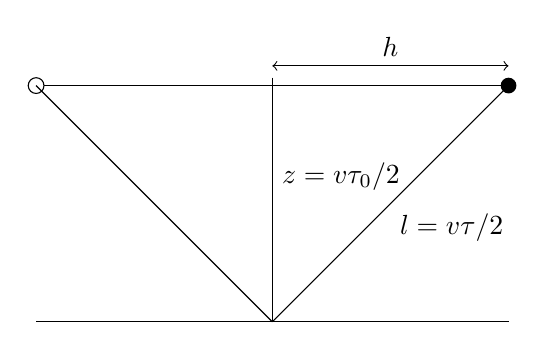
\begin{tikzpicture}
  \draw (0.0,1.0) -- (6.0,1.0) ;
  \draw (0.0,4.0) -- (6.0,4.0) ;
  \draw[<->](3.0,4.25) -- node[above]{$h$}(6.0,4.25) ;
  \fill[white] (0.0,4.0) circle (0.1) ;
  \draw (0.0,4.0) circle (0.1) ;
  \fill (6.0,4.0) circle (0.1) ;
  \draw (6.0,4.0) -- node[below right]{$l=v\tau/2$}(3.0,1.0) ;
  \draw (3.0,1.0) -- (0.0,4.0) ;
  \draw (3.0,4.1) -- node[above right]{$z=v\tau_0/2$}(3.0,1.0) ;
\end{tikzpicture}
\label{fig:nmop}
\end{figure}

The traveltime $\tau(h)$ is:
%
\begin{eqnarray}
l^2 = z^2+h^2 \nonumber\\
\end{eqnarray}
which gives by inserting $v\tau/2$ for $l$ and $v\tau_0/2$ for $z$
\begin{eqnarray}
\tau(h)=\sqrt{t^2_0+4h^2/v^2}.
\label{eq:nmo}
\end{eqnarray}
\end{frame}
%-----------------------------------------
\begin{frame}{NMO and Stack}
%-----------------------------------------
Nmo-correction:
%
\begin{eqnarray}
 \Delta \tau = \tau(h)-\tau_0,
\label{eq:dtnmo}
\end{eqnarray}
\end{frame}
%
%-----------------------------------------
\begin{frame}{Cmp}
%-----------------------------------------
\begin{figure}
 \includegraphics[width=0.50\textwidth]{Fig/synshot.pdf}
\end{figure}
\end{frame}
%-----------------------------------------
\begin{frame}{Nmo}
%-----------------------------------------
\begin{figure}
 \includegraphics[width=0.50\textwidth]{Fig/syncmp.pdf}
\end{figure}
\end{frame}
%-----------------------------------------
\begin{frame}{Stack}
%-----------------------------------------
\begin{figure}
 \includegraphics[width=0.50\textwidth]{Fig/synstack.pdf}
\end{figure}
\end{frame}
%-----------------------------------------
\begin{frame}{NMO and Stack}
%-----------------------------------------
Average velocity $v_{rms}$ defined by
\begin{eqnarray}
 v^2_{rms}(t_0)=\frac{1}{t_0}\int^{t_0}_0 v^2(t)dt
\label{eq:rms}
\end{eqnarray}
$v(t)$ : Interval velocity.
The traveltime equation \eqref{eq:nmo} then becomes
\begin{eqnarray}
\tau(h)=\sqrt{t^2_0+4h^2/v^2_{rms}(t_0)}.
\label{eq:nmorms}
\end{eqnarray}
\end{frame}
%-----------------------------------------
\begin{frame}{Velocity analysis}
%-----------------------------------------
%
  Estimate $v_{rms}$ from equation \eqref{eq:nmo}
\begin{enumerate}
  \item Make a guess of $v$ 
  \item Perform Nmo correction for all $t_0$ with using guess of $v$
  \item Make a stack trace
  \item Perform above steps for a range of guesses of $v$
  \item Plot all stack traces in a velocity spectrum
\end{enumerate}
\end{frame}
%-----------------------------------------
\begin{frame}{Velocity spectrum}
%-----------------------------------------
\begin{figure}
 \includegraphics[width=0.50\textwidth]{Fig/synscn.pdf}
\end{figure}
\end{frame}
%-----------------------------------------
\begin{frame}{Semblance}
%-----------------------------------------
Stack is usually replaced with semblance to
get better velocity spectra  
\begin{eqnarray}
S(t) = \frac{\int_0^{h_{max}} p^2(t,h)}{\int dt_0^T\, \int_0^{h_{max}} p^2(t,h)}
\end{eqnarray}
\begin{itemize}
 \item $p(t,h)$ : data 
 \item $h_{max}$: maximum offset. 
\end{itemize}
This equation can not be used directly.  Why?
\end{frame}
%
%-----------------------------------------
\begin{frame}{Semblance}
%-----------------------------------------
\begin{eqnarray}
S_k = \frac{\sum_{i=0}^{N_h} p^2_{k,i}}{\sum_{k=0}^{N_t} \sum_{i=0}^{N_h} p^2_{k,i}}
\end{eqnarray}
\begin{itemize}
 \item $S_k = S(t=k\Delta t), k=0,\ldots,N_t$ 
 \item $p_{k,i}=p(t=k\Delta t,h=i\Delta h), i=0,\ldots,N_h$. 
 \item $\Delta t$ time sampling interval, 
 \item $\Delta h$ distance between offsets \item $N_t$,$N_h$ :
No of time samples and No of  offsets
\end{itemize}
\end{frame}
%-----------------------------------------
\begin{frame}{Velocity analysis}
%-----------------------------------------
\begin{figure}
 \includegraphics[width=0.50\textwidth]{Fig/synvel.pdf}
\end{figure}
\end{frame}
%-----------------------------------------
\begin{frame}{Velocity analysis}
%-----------------------------------------
\begin{figure}
 \includegraphics[width=0.50\textwidth]{Fig/cmp.pdf}
\end{figure}
\end{frame}
%-----------------------------------------
\begin{frame}{Velocity analysis}
%-----------------------------------------
\begin{figure}
 \includegraphics[width=0.50\textwidth]{Fig/scn-1.pdf}
\end{figure}
\end{frame}
%-----------------------------------------
\begin{frame}{Velocity analysis}
%-----------------------------------------
\begin{figure}
 \includegraphics[width=0.50\textwidth]{Fig/nmo.pdf}
\end{figure}
\end{frame}
%-----------------------------------------
\begin{frame}{Velocity analysis}
%-----------------------------------------
\begin{figure}
 \includegraphics[width=0.50\textwidth]{Fig/stack.pdf}
\end{figure}
\end{frame}
%--------------------------------------------
\begin{frame}{Summary}
%--------------------------------------------
\begin{itemize}
  \item Seismic data acquisition
   \item CMP method
   \item NMO-correction
   \item Velocity analysis
  \end{itemize}
%
\end{frame}

%==============================================
\begin{frame}{Overview}
%==============================================
\begin{itemize}
  \item Migration principles
  \item Kirchhoff Time migration
\end{itemize}
\end{frame}
%==============================================
\begin{frame}{Migration principles}
%==============================================
%
\begin{figure}
\begin{tikzpicture}[scale=1.5]
  \draw[->] (-0.5,4.0) -- (-0.5,0.0) node[below]{Depth} ;
  \draw[<->] (1.0,5.0) -- node[fill=white]{Offset} (5.0,5.0); 
  \draw (0.0,0.0) -- (6.0,0.0) ;
  \draw (0.0,4.0) -- (6.0,4.0) ;
  \fill (5.0,4.0) node[above]{Source} circle (0.1) ;
  \fill[white] (0.0,4.0) circle (0.1) ;
  \draw (0.0,4.0) circle (0.1) ;
  \fill[white](1.0,4.0) circle (0.1) ;
  \draw (1.0,4.0) node[above]{Receiver}circle (0.1) ;
  \fill[white] (2.0,4.0) circle (0.1) ;
  \draw (2.0,4.0) circle (0.1) ;
  \fill[white] (3.0,4.0) circle (0.1) ;
  \draw (3.0,4.0) circle (0.1) ;
  \fill[white] (4.0,4.0) circle (0.1) ;
  \draw (4.0,4.0) circle (0.1) ;
  \draw (5.0,4.0) -- (3.0,0.0) ;
  \draw (3.0,0.0) -- (1.0,4.0) ;
% Upgoing wave circle
  \draw (3,0) +(80:3) arc(80:152:3);
  \draw (3,0) +(0:0.25) arc(0:180:0.25);
  \draw (5,4) +(-80:3) arc(-80:-152:3);
  \draw (5,4) +(-90:4.47) arc(-90:-142:4.47);
  \draw (5.0,1.5) node[right]{$D$};
  \draw (0.5,2.0) node[left]{$U$};
  \draw (3,0) node[below]{$R$};
  \draw[->] (3,0)-- +(116:1);
\end{tikzpicture}
\label{fig:si-1}
\end{figure}
\end{frame}
%==============================================
\begin{frame}{Migration principles}
%==============================================
\begin{figure}
\begin{tikzpicture}[scale=1.5][stealth]
  \draw[->] (-0.5,4.0) -- (-0.5,0.0) node[below]{Depth} ;
% \draw[<->] (1.0,5.0) -- node[fill=white]{Offset} (5.0,5.0); 
  \draw (0.0,0.0) -- (6.0,0.0) ;
  \draw (0.0,4.0) -- (6.0,4.0) ;
  \fill (5.0,4.0) node[above]{Source} circle (0.1) ;
  \fill[white] (0.0,4.0) circle (0.1) ;
  \draw (0.0,4.0) circle (0.1) ;
  \fill[white](1.0,4.0) circle (0.1) ;
  \draw (1.0,4.0) node[above]{Receiver}circle (0.1) ;
  \fill[white] (2.0,4.0) circle (0.1) ;
  \draw (2.0,4.0) circle (0.1) ;
  \fill[white] (3.0,4.0) circle (0.1) ;
  \draw (3.0,4.0) circle (0.1) ;
  \fill[white] (4.0,4.0) circle (0.1) ;
  \draw (4.0,4.0) circle (0.1) ;
  \draw (5.0,4.0) -- (3.0,0.0) ;
% \draw (3.0,0.0) -- (1.0,4.0) ;
% Upgoing wave circle
  \draw (3,0) +(0:0.25) arc(0:180:0.25);
  \draw (5,4) +(-90:4.47) arc(-90:-142:4.47);
  \draw (4.5,-0.2) node[right]{$D$};
  \draw (3.0,0.5) node[above]{$U$};
  \draw (3,0) node[below]{$R$};
  \draw[->] (3,0)-- +(116:1);
\end{tikzpicture}
\label{fig:si-2}
\end{figure}
%
\end{frame}
%==============================================
\begin{frame}{Migration principles}
%==============================================
Make an image by cross-correlating the downgoing
and upgoing waves
\begin{eqnarray}
 R(\mathbf{x})=\int dt U(\mathbf{x},t)D(\mathbf{x},t),
   \label{eq:si-1}
\end{eqnarray}
where $R$ is the reflectivity and $\mathbf{x}=(x,y,z)$ denotes
a position in space, while $t$ is the time.
\end{frame}
%==============================================
\begin{frame}{Kirchhoff migration}
%==============================================
Simplest approach for up- and downgoing waves
\begin{eqnarray}
  D(\mathbf{x},t)=A \delta(t-\tau_s),\nonumber\\
  U(\mathbf{x},t)=B P(t+\tau_r),
   \label{eq:si-2}
\end{eqnarray}
where
\begin{itemize}
\item $\mathbf{x}$: reflection point, 
\item $A$ and $B$: amplitude factors
\item $P$: Data at the surface
\item $\tau_s$ traveltime from the source to the reflection point 
\item $\tau_s$ traveltime from the receiver to the reflection point 
\end{itemize}
\end{frame}
%==============================================
\begin{frame}{Kirchhoff migration}
%==============================================
Using equation \eqref{eq:si-2} and equation \eqref{eq:si-1}, I get
%
\begin{eqnarray}
 R(\mathbf{x})=\int dt A \delta(t-\tau_s)B P(t+\tau_r),
   \label{eq:si-3}
\end{eqnarray}
which after integration gives
\begin{eqnarray}
 R(\mathbf{x})= AB P(\tau_s+\tau_r).
   \label{eq:si-4}
\end{eqnarray}
%
If we disregard the amplitude factor $AB$ the image is simply equal to 
the amplitude of the recorded data at a time equal to $\tau=\tau_r+\tau_s$.
\end{frame}
%==============================================
\begin{frame}{Kirchhoff migration}
%==============================================
%
\begin{figure}
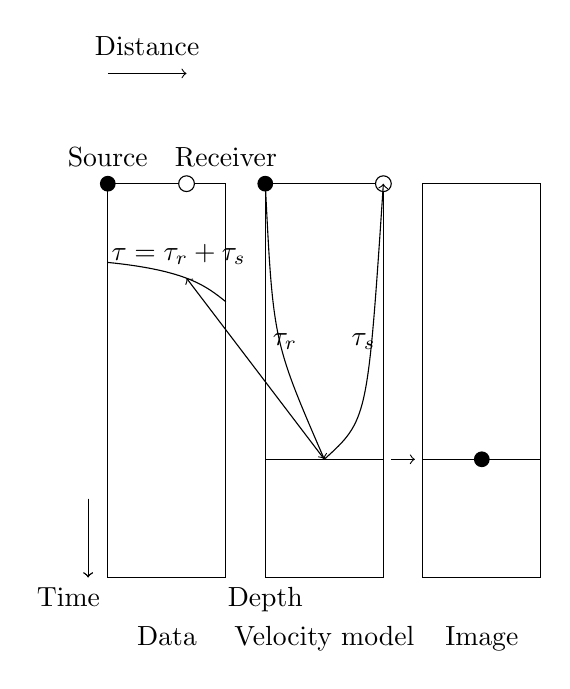
\begin{tikzpicture}[scale=1.0][stealth]
% Time section  
  \draw (0,0) rectangle +(1.5,5);
  \fill (0.0,5.0) circle (0.1) ;
  \draw (0.0,5.1) node[above]{Source};
  \fill[white] (1.0,5.0) circle (0.1) ;
  \draw (1.0,5.0) circle (0.1) ;
  \draw (1.5,5.1) node[above]{Receiver};
  \draw (0,4) .. controls (1.0,3.9) and (1.25,3.7).. (1.5,3.5);
  \draw (0.5,6.5) node[above]{Distance};
  \draw (-0.5,0) node[below]{Time};
  \draw[->] (0,6.4) -- (1,6.4);  
  \draw[->] (-0.25,1) -- (-0.25,0);  
  \draw (0.75,-0.5) node[below]{Data};
% Depth model
  \draw (2,0) rectangle +(1.5,5);
  \fill (2,0) +(0.0,5.0) circle (0.1) ;
  \fill[white] (2,0) +(1.5,5.0) circle (0.1) ;
  \draw (2,0) +(1.5,5.0) circle (0.1) ;
  \draw (2.0,0) node[below]{Depth};
  %\draw[->] (0,5.5) -- (1,5.5);  
  \draw[->] (-0.25,1) -- (-0.25,0);  
%
% Rays
% \draw[->] (2.0,5) -- (2.75,1.5);
% \draw[->] (2.75,1.5) -- (3.5,5);
  \draw[->] (2.0,5) .. controls (2.1, 3) ..(2.75,1.5);
  \draw[->] (2.75,1.5) .. controls (3.3,2.0) .. (3.5,5);
%
  \draw (2.0,1.5) -- (3.5,1.5);
  \draw (2,0) +(0.75,-0.5) node[below]{Velocity model};
  \draw (2,0) +(1.25,3) node{$\tau_s$};
  \draw (2,0) +(0.25,3) node{$\tau_r$};
  \draw[->] (2.75,1.5) -- (1.0,3.8);
  \draw (0.9,4.1) node{$\tau=\tau_r+\tau_s$};
% Image
  \draw[->] (3.6,1.5) -- (3.9,1.5);
  \draw (4,0) rectangle +(1.5,5);
  \draw (4,0) +(0.75,-0.5) node[below]{Image};
  \draw (4.0,1.5) -- +(1.5,0);
  \fill (4.75,1.5) circle (0.1) ;
\end{tikzpicture}
\caption{Kirchhoff depth migration}
\label{fig:si-3}
\end{figure}
\end{frame}
%==============================================
\begin{frame}{Kirchhoff migration}
%==============================================
Many source-receiver pairs will contribute to the same imaging point, so
that equation \eqref{eq:si-4} becomes
\begin{eqnarray}
 R(\mathbf{x})= \sum_{r,s}P(\tau_s+\tau_s),
   \label{eq:si-5}
\end{eqnarray}
where we have neglected the amplitude factors and the summation is
over all source-receiver pairs contributing to the image point.
\end{frame}
%==============================================
\begin{frame}{Kirchhoff migration}
%==============================================
%
\begin{figure}
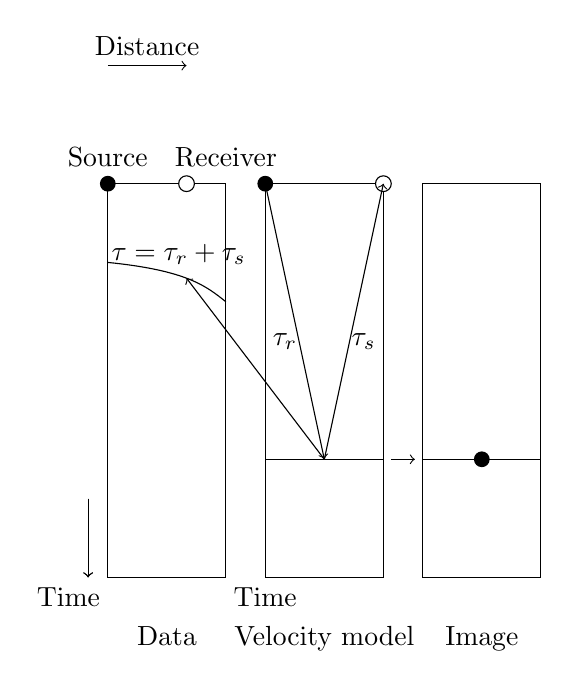
\begin{tikzpicture}[scale=1.0][stealth]
% Time section  
  \draw (0,0) rectangle +(1.5,5);
  \fill (0.0,5.0) circle (0.1) ;
  \draw (0.0,5.1) node[above]{Source};
  \fill[white] (1.0,5.0) circle (0.1) ;
  \draw (1.0,5.0) circle (0.1) ;
  \draw (1.5,5.1) node[above]{Receiver};
  \draw (0,4) .. controls (1.0,3.9) and (1.25,3.7).. (1.5,3.5);
  \draw (0.5,6.5) node[above]{Distance};
  \draw (-0.5,0) node[below]{Time};
  \draw[->] (0,6.5) -- (1,6.5);  
  \draw[->] (-0.25,1) -- (-0.25,0);  
  \draw (0.75,-0.5) node[below]{Data};
% Depth model
  \draw (2,0) rectangle +(1.5,5);
  \fill (2,0) +(0.0,5.0) circle (0.1) ;
  \fill[white] (2,0) +(1.5,5.0) circle (0.1) ;
  \draw (2,0) +(1.5,5.0) circle (0.1) ;
  \draw (2.0,0) node[below]{Time};
  %\draw[->] (0,5.5) -- (1,5.5);  
  \draw[->] (-0.25,1) -- (-0.25,0);  
%
% Rays
 \draw[->] (2.0,5) -- (2.75,1.5);
 \draw[->] (2.75,1.5) -- (3.5,5);
%
  \draw (2.0,1.5) -- (3.5,1.5);
  \draw (2,0) +(0.75,-0.5) node[below]{Velocity model};
  \draw (2,0) +(1.25,3) node{$\tau_s$};
  \draw (2,0) +(0.25,3) node{$\tau_r$};
  \draw[->] (2.75,1.5) -- (1.0,3.8);
  \draw (0.9,4.1) node{$\tau=\tau_r+\tau_s$};
% Image
  \draw[->] (3.6,1.5) -- (3.9,1.5);
  \draw (4,0) rectangle +(1.5,5);
  \draw (4,0) +(0.75,-0.5) node[below]{Image};
  \draw (4.0,1.5) -- +(1.5,0);
  \fill (4.75,1.5) circle (0.1) ;
\end{tikzpicture}
\caption{Kirchoff time migration}
\label{fig:si-4}
\end{figure}
\end{frame}
%
%==============================================
\begin{frame}{Kirchhoff migration}
%==============================================
Assume velocity $c(\mathbf{x})$ is depth
dependent only, $c=c(z)$, then

\begin{eqnarray}
\tau_s = \sqrt{\frac{(x-x_s)^2+(y-y_s)^2}{c^2} + \tau^2_0} ,\nonumber\\
\tau_r = \sqrt{\frac{(x-x_r)^2+(y-y_r)^2}{c^2}+\tau^2_0} ,
\end{eqnarray}
\begin{itemize}
\item $(x_r,y_r)$, $(x_s,ys)$: Source, receiver positions
\item $\tau_0=z/c$ :vertical traveltime and 
\item $c$ : velocity.
\end{itemize}
\end{frame}
%==============================================
\begin{frame}{Kirchhoff migration}
%==============================================
We then get for the total traveltime $\tau$ 
\begin{eqnarray}
 \tau=\sqrt{\frac{(x-x_s)^2+(y-y_s)^2}{c^2}+\tau^2_0}+ \sqrt{\frac{(x-x_r)^2+(y-y_r)^2}{c^2}+\tau^2_0}.
\label{eq:si-7}
\end{eqnarray}
The image $R$ is then
\begin{eqnarray}
 R(x,y,\tau_0)= \sum_{r,s}P(\tau_s+\tau_s),
   \label{eq:si-8}
\end{eqnarray}
\end{frame}
%==============================================
\begin{frame}{Zero-offset simple migration}
%==============================================
We get for zero-offset (stack) data
(2D)
\begin{eqnarray}
 \tau=2\sqrt{\frac{(x-x_s)^2}{c^2}+\tau^2_0}.
\label{eq:si-7}
\end{eqnarray}
\end{frame}
%==============================================
\begin{frame}{Zero-offset simple migration}
%==============================================
Migration of zero-offset section can then be done as:
\begin{itemize}
   \item Chose a point $x_s,\tau_0$ on the section.
   \item Loop over all $x$ values, compute $\tau$ and sum
         all $P(\tau)$ (Summing over an hyperbola
         with center at $x_s,\tau_0$.)
   \item Put the sum at location $x_s,\tau_0$ in the output.
   \item Repeat for all possible points $x_s,\tau_0$.
\end{itemize}
\end{frame}
%==============================================
\begin{frame}{Basic+ processing sequence}
%==============================================
\begin{enumerate}
  \item Input data
  \item Velocity analysis
  \item NMO + Stack
  \item Zero-offset (poststack) migration,
  \item Output result
\end{enumerate}
Nobody with full possession of their faculties uses 
a processing sequence like this today, except for initial QC.
\end{frame}
%=================================================
\begin{frame}{Basic++ processing sequence (time)}
%=================================================
\begin{enumerate}
  \item Input data
  \item preprocessing (designature, debubble, etc..)
  \item Multiple removal
  \item Initial prestack migration
  \item Velocity analysis on demigrated data.
  \item Final prestack migration
  \item Multiple removal
  \item Stack
  \item Output result
\end{enumerate}
\end{frame}
\end{document}
